\documentclass{report}
\usepackage{graphicx}
%%%%%%%%%
%%%%%%%%% WARNING: THIS DOCUMENT IS IN THE PROCESS OF REVISION AND MAY
%%%%%%%%% CURRENTLY BE WILDLY INACCURATE.
%%%%%%%%%

% Begin title and author information (Come up with a better title :)
\title{OVM: Repository Documentation}
\author{Krista Bennett, Christian Grothoff, Krzysztof Palacz, Jan Vitek}
\date{\today}
% End title and author information

%
% ALSO NOTE: In places I have borrowed liberally from the documentation
% already in the code. I don't know who wrote what, so it may be decided
% later that the author list should be all-inclusive, absent, or simply
% listed as ``The OVM development team''.
%
% For the time being, I have put the list in alphabetical order, including
% all of the authors from any file I took comments from that I know I
% didn't write myself. Please add or delete as necessary; I do not
% intend anything other than to give credit where credit is due! - klb
%

\begin{document}
\maketitle
\tableofcontents
\newpage
\chapter{Introduction}
This document describes the component of OVM known as the 
{\em repository}. The repository is a structure which contains the 
an object-oriented representation of the information contained in Java 
\texttt{.class} files. This representation is shared across domains to allow 
the bytecode of a class to be used by several applications without having to 
reload the class definition. Repository data structures are read-only; 
modifications of this shared data are not allowed.

Not all of the descriptions provided in this document are implementation 
specific; the commentary is meant to describe the repository interfaces and
classes which should be common to all implementations. 
Implementations may choose to augment this functionality as appropriate.

It should be noted that the explanations in this document are not intended
to replace an understanding of concepts referred to in the JVM Specification
\cite{LindholmY96}. While this document does often contain brief summaries of 
such concepts when it seems necessary to clarify usage or explain how these 
concepts are realized in OVM, the reader should refer to the JVM Specification
for further information about general VM-related questions when appropriate.

\section{Overview of the Repository}

The repository, as mentioned previously, is shared across domains. 
Domains are not discussed in detail within this document; however, it 
should be noted that a domain is primarily an application space. In general, 
applications running in different domains have no interactions via shared 
objects (note that since the repository is not modified by applications, 
{\em interactions} between applications in different domains will not occur 
via shared repository data). Separate domains can have different 
implementations of the same class. The domain with which an application is 
associated will determine where classes will be searched for.

The repository itself consists of many different components 
(fig. \ref{repos_graphic}). To begin with,
the repository contains data structures which represent all of the information 
obtained by parsing individual Java class files. The top-level objects are 
instances of \texttt{Re\-pos\-i\-tory\-Class}. These 
\texttt{Re\-pos\-i\-tory\-Class} objects, then, are grouped into bundles
through instances of the \texttt{Bundle} class which are used by the domain to
determine the correct \texttt{Re\-pos\-i\-tory\-Class} to load when a class is 
referenced. This is particularly useful when there are multiple 
implementations of a particular class in the system. At a first approximation,
bundles can be viewed as supporting functionality similar to that of a 
classloader with respect to namespace management.

\begin{figure}[htb]
\begin{center}
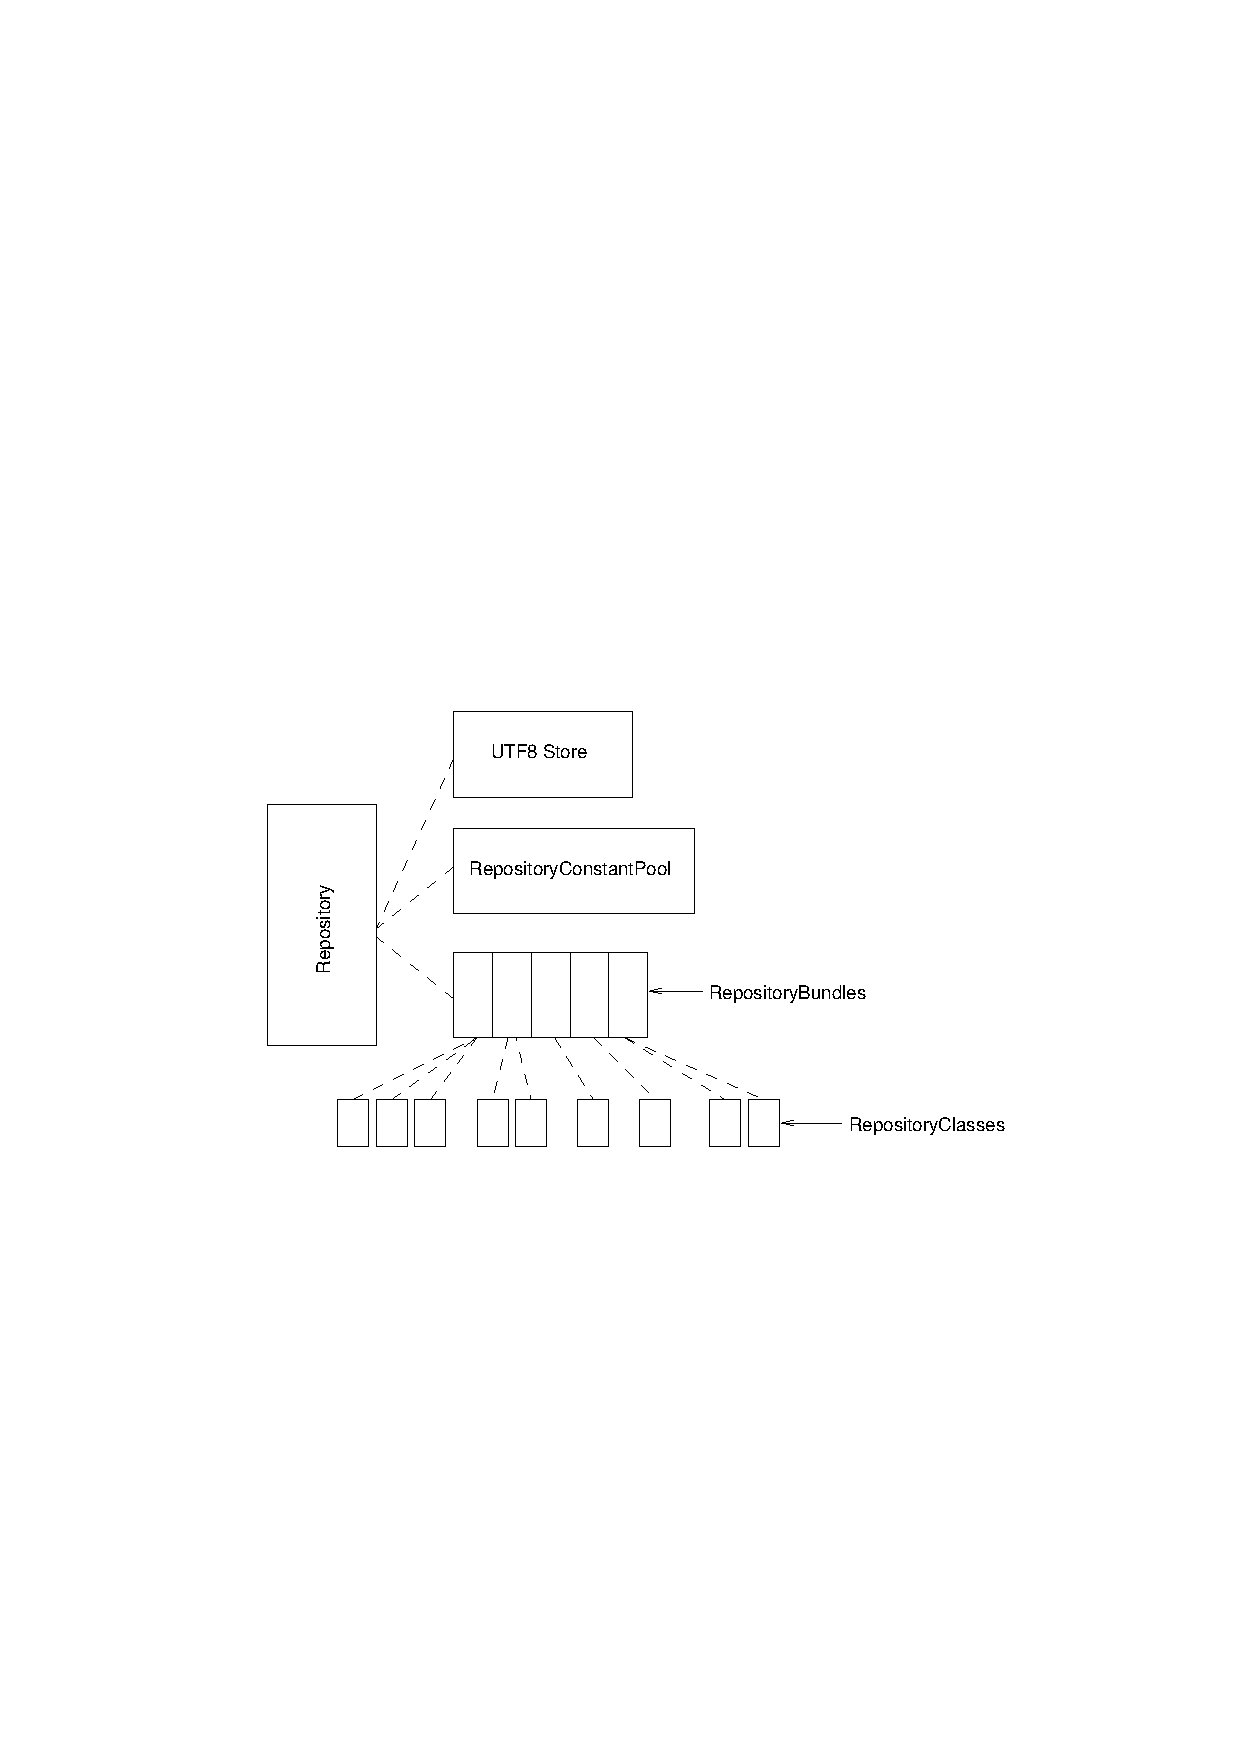
\includegraphics{repository_comp.epsi}
\caption{Some basic components of the repository}
\label{repos_graphic}
\end{center}
\end{figure}

\texttt{RepositoryClass} objects contain component objects which encapsulate
different kinds of information found within a class file. There is information
which relates to the class itself, such as the name of the class and its
modifiers, as well as information relating to its member fields, methods,
classes, interfaces, etc. This is not a complete list of everything contained
in a \texttt{Re\-pos\-i\-tory\-Class}; for further detail, see \S 
\ref{repclass}.

\section{Structure of this document}
This document is divided into three main parts. Chapter \ref{components}
describes the objects that make up the repository. Chapter \ref{usage} 
explains how these objects can be created and used, along with any general
usage issues that may be related to a particular component. Finally, Chapter 
\ref{defs} provides definitions of terms that are used in the text for
quick reference.

\chapter{Repository Components and Structure}\label{components}

The repository itself is made up of many interrelated components. This
chapter aims to describe each component's function, structure, and relationship
to other objects within the repository. Note that this information
is primarily descriptive; for functional information, please see Chapter
\ref{usage}.

%Please note that when class diagrams appear in this section, they do {\em not}
%contain the full functionality of the class. Rather, they are intended to 
%demonstrate the described components of the class. There may be additional
%methods within the class which are not displayed or described.

\section{The Utf8 Store}\label{utf8store}

The utf8 store is an object used for storage and retrieval of utf8 character
strings within the repository. Strings that do not currently exist in the
utf8 store are {\em installed} there. These can then later be retrieved
via their utf8 store index. Multiple occurances of the same character string
will be shared (i.e. located at the same index). The \texttt{utf8Store}
contains methods for installing these strings as well as retrieving them
as utf8 store indices, \texttt{String} objects, or writing them to an
output stream. Properties such as string length can also be ascertained.

\section{Bundle}

A \texttt{Bundle} is a logical grouping of 
\texttt{Re\-pos\-i\-tory\-Classes}. Bundles occur in a hierarchy which is used
by the domain context to determine which \texttt{Re\-pos\-i\-tory\-Classes} 
should be loaded at particular points in time (see \S \ref{repclass} for
the description of the \texttt{Re\-pos\-i\-tory\-Class} data structure).

Classes are installed into the repository via whichever bundle they are 
intended to become a member of. If, when attempting to install a new class, a 
class with the same name, version and hash value already exists in the 
repository, the duplicate class is not added to the bundle. 
Classes may be added to a bundle until that bundle is {\em sealed}.
Sealing effectively makes a bundle immutable and will cause exceptions to
be thrown if further attempts to install classes via a given bundle occur.

\medskip

{\em N.B. Bundle is not fully fleshed-out and may change dramatically}
% FIXME: Still true?

\section{ConstantPool}\label{pool}

Each \texttt{RepositoryClass} object has a reference to a constant pool
which contains symbolic information about repository structures which the 
virtual machine will need at runtime. This constant pool
is maintained in a \texttt{Con\-stant\-Pool} object. 
The constant pool is described in the JVM Specification, \S 4.4.

The constant pool is essentially a table; each entry consists of a 
tag/infor\-mation pair: the tag indicates what constant type is being referred
to, and its information is constant-specific information which varies depending
upon the tag.

%All non-primitive constant pool entries must implement 
%\texttt{Con\-stant\-Pool.En\-try}.

%Implementations of \texttt{RepositoryConstantPool.Entry} are non-primitive
%constant pool objects. Such objects include \texttt{Se\-lec\-tors},
%\texttt{RepositoryDescriptors}, and \texttt{TypeNames}.

% FIXME: Are these still around somewhere?

\section{RepositoryClass}\label{repclass}

\texttt{RepositoryClass} objects represent the class information for
individual classes within the repository as obtained from \texttt{.class}
files. These objects represent both classes and interfaces. They contain
the data structures and interfaces necessary to access and manipulate
class components. 

A \texttt{RepositoryClass} object is made up of several components (these are
displayed in table \ref{class_table}). Some
of these relate directly to the class this \texttt{Re\-pos\-i\-tory\-Class} 
represents. First of all, there is a \texttt{TypeName.Scalar} object which 
gives the name of this class with references to both the class's simple name 
and the class's package name (\S \ref{typename}). There is also a 
\texttt{Mode} object (\S \ref{mode}) which contains the modifiers for this 
class, as well as an array of attribute objects (\S \ref{attrib}) containing 
this class's attributes. In reference to the \texttt{.class} file itself, the 
major and minor versions of the class file that generates a given 
\texttt{Re\-pos\-i\-tory\-Class} are stored within the object as well.

A reference to the \texttt{TypeName} of this class's super class is also 
contained within the object; this is a self-referrential link for the root of 
the hierarchy (i.e. \texttt{java.lang.Object} in Java). All
\texttt{Re\-pos\-i\-tory\-Class} objects also have a reference to their 
enclosing class. If a \texttt{Re\-pos\-i\-tory\-Class} object does not 
represent an inner class, this reference remains \texttt{null}. There is also
an array of \texttt{TypeName} objects maintained which represents the 
{\em linkset} of this class -- these are the classes and interfaces 
required by the class's implementation.

\begin{table}
\begin{center}
\begin{small}
\begin{tabular}{l l} 
	Component & Representation Type \\ \hline
 	{\em name}: & \texttt{TypeName.Scalar} \\
	{\em modifiers}: & \texttt{Mode.Class}  \\	 
 	{\em attributes}: & \texttt{Attribute[]} \\
 	{\em interfaces}: & \texttt{TypeName.Scalar[]} \\
 	{\em super class}: & \texttt{TypeName.Scalar} \\
 	{\em outer class}: & \texttt{TypeName.Scalar} \\
 	{\em component type}: & \texttt{TypeName} \\
 	{\em linkset}: & \texttt{TypeName.Compound[]} \\
	{\em constant pool}: & \texttt{ConstantPool} \\
 	{\em major version}: & \texttt{int} \\
 	{\em minor version}: & \texttt{int} \\ %\hline
	{\em static fields:} & 	\texttt{RepositoryMember.Field[]} \\
	{\em instance fields:} & \texttt{RepositoryMember.Field[]} \\
	{\em static methods:} & \texttt{RepositoryMember.Method[]} \\
	{\em instance methods:} & \texttt{RepositoryMember.Method[]} \\ 
	{\em static inner classes:} & \texttt{TypeName.Scalar[]} \\
	{\em instance inner classes:} & \texttt{TypeName.Scalar[]} \\
\end{tabular}
\end{small}
\caption{Important components of a \texttt{RepositoryClass} object}
\label{class_table}
\end{center}
\end{table}

%\begin{figure}[htb]
%\begin{center}
%\includegraphics{class_comp.epsi}
%\caption{Important components of a \texttt{RepositoryClass} object}
%\label{class_graphic}
%\end{center}
%\end{figure}

As would also be expected, there are references to objects representing the 
members of a class. Methods and fields are contained within the
\texttt{Repository\-Class} object in arrays of 
\texttt{Re\-pos\-i\-tory\-Mem\-ber.Meth\-od} and 
\texttt{RepositoryMem\-ber.Field} respectively. Distinctions are made
between static and instance members, and both can be retrieved via the
corresponding \texttt{Re\-pos\-i\-tory\-Class}. There is also functionality to
retrieve methods and fields for a class using a representation of the 
corresponding unbound selector (see \S \ref{unbound} for information on 
unbound selectors); these require existing knowledge of a method or field's
name and type information. 

There are also references within the object to static and instance inner 
classes through their corresponding \texttt{TypeName} objects. Declared
implemented interfaces are stored similarly, as \texttt{TypeName} arrays,
and can be retrieved as such. 

Finally, there is a reference to the class constant pool, which contains
all of the constants referenced in the class (see \S \ref{pool} for
more information).

All of these structures should be made available through
\texttt{Re\-pos\-i\-tory\-Class} methods. Subsequent sections explain the 
components make up the \texttt{Repository\-Class} structure.

\newpage

\section{TypeName}\label{typename}

\texttt{TypeName} objects describe the name of a Java object type
(class or interface) obtained from a class file. There are several
different categories of \texttt{TypeName} objects, all of which correspond
to the type they represent. Their relationships to one another are shown in 
figure \ref{type_graphic} and described in detail in the rest of this section.

\begin{figure}[htb]
\begin{center}
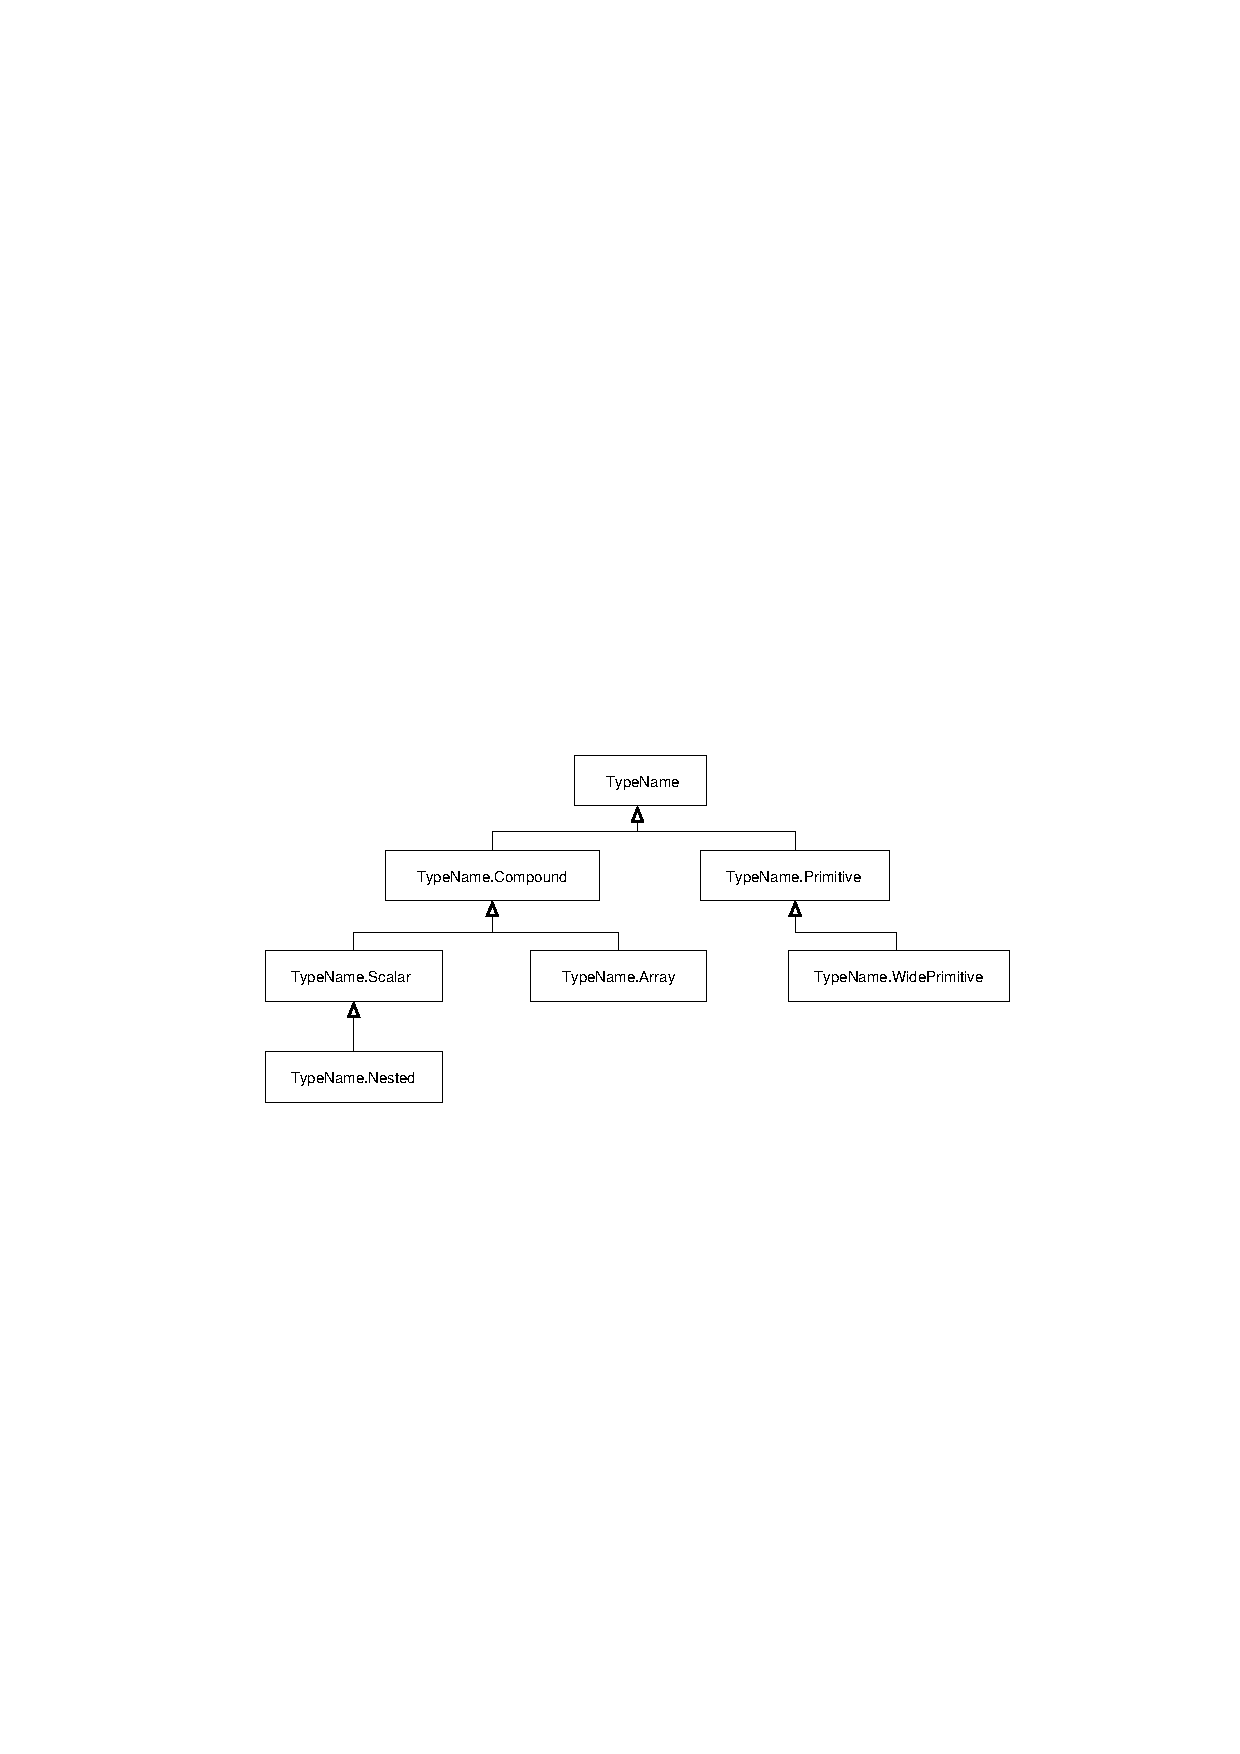
\includegraphics{typehierarchy.epsi}
\caption{The hierarchy of \texttt{TypeName} classes}
\label{type_graphic}
\end{center}
\end{figure}

\subsection{Common Structure}\label{type_common}

% FIXME: This looks ugly.

All \texttt{TypeName} objects should contain several pieces of information 
(see table \ref{typename_table}).
First of all, they should contain the repository utf8 string index of
the simple type name the object is supposed to represent.  This name is the 
unqualified name of the type as specified in its class file - for example,
\texttt{Object}, not \texttt{Ljava\//lang\//Object;}. (See JVM Specification,
\S 2.7, for more information on simple names). 
Secondly, they should contain the \texttt{char} representing the type tag, 
or \texttt{TypeCodes} constant, for this type. This will indicate whether 
this is type for a reference object, a particular type of primitive 
(\texttt{int} vs. \texttt{boolean}, etc.), an array, etc. There is also a 
method to return the fully 
qualified type name as a \texttt{String} object. This is a string containing 
the full type and package name, and if this is an array, the proper number of 
leading brackets (e.g. \texttt{[[Ljava\//lang\//Object;} as a representation of
a two-dimensional array of \texttt{Object}). In addition to 
being able to return this name as a \texttt{String}, there should also be a
mechanism for writing the fully qualified name to a given output stream. 
Finally, there should be a record of the length of the \texttt{TypeName}
object's fully-qualified name string. For primitive types, this should always
be $1$ (see \S \ref{primtype} for more explanation).

\begin{table}
\begin{center}
\begin{small}
\begin{tabular}{l l} 
	Component & Representation Type \\ \hline
	{\em simple name index}: & \texttt{int} \\
	{\em type tag}: & \texttt{char} \\
	{\em fully qualified type name}: & \texttt{String} \\
\label{typename_table}
\end{tabular}
\end{small}
\caption{Important components of the basic \texttt{TypeName} object}
\end{center}
\end{table}

%\begin{figure}[htb]
%\begin{center}
%\includegraphics{TypeName.epsi}
%\caption{The basic functionality of \texttt{TypeName}}
%\label{type_typename}
%\end{center}
%\end{figure}

\subsection{Primitive TypeNames}\label{primtype}

\texttt{TypeName.Primitive} objects represent the type names of
primitive types, as the name suggests. There are two types of
primitive typenames: \texttt{Type\-Name.Prim\-i\-tive} objects which
are not instances of \texttt{Type\-Name.Wide\-Prim\-i\-tive} are generally
reserved for types of one-word length. \texttt{Type\-Name.Wide\-Prim\-i\-tive}
objects, then, are for types of two-word length. 

% Implementations of primitive type names only require the functionality 
% specified for generic \texttt{TypeName} objects. 
%(see fig. \ref{type_primitive}).

%\begin{figure}[htb]
%\begin{center}
%\includegraphics{Primitive.epsi}
%\caption{The basic functionality of \texttt{TypeName.Primitive}}
%\label{type_primitive}
%\end{center}
%\end{figure}

As mentioned previously, the name length returned by the \texttt{length()} 
method for a primitive type name will always be $1$. This is because the 
contents of the name string for primitive type names is the corresponding 
\texttt{TypeCodes} character constant (see \S \ref{typecodes}).

\subsection{Compound TypeNames}

% FIXME: Gemeinsam, etc.

\texttt{TypeName.Compound} objects represent the type names of all
non-primitive types. This includes the \texttt{TypeName.Scalar} type names,
which are used for all non-primitive, non-array types, and 
\texttt{TypeName.Array} type names for arrays. The \texttt{Scalar} type name
interface also contains a subinterface which is used for nested interface or 
class type names (\texttt{TypeName.Nested}).

%As shown in figure \ref{type_compound}, 
Compound \texttt{TypeName} classes 
must implement two pieces of functionality
in addition to that which is required for generic \texttt{TypeName} objects. 
First of all, they must have some reference to the repository utf8 index of the
package name of which the class is a member, as well as a method to retrieve 
this. Secondly, there must be a method to return the \texttt{String} 
representation of the type name as required in the 
\texttt{CONSTANT\_Class\_info} bytecode structure (see JVM Specification, 
\S 4.2). This is the fully qualified name, but without the leading 'L' in the 
case of \texttt{Scalar} type names.

%\begin{figure}[htb]
%\begin{center}
%\includegraphics{Compound.epsi}
%\caption{The basic functionality of \texttt{TypeName.Compound}}
%\label{type_compound}
%\end{center}
%\end{figure}

%% FIXME - more here.

%% FIXME: Make sure this definition is correct. Fully-qualified is bandied 
%% about a lot in the code, and sometimes it isn't really what's being 
%% specified, but some weird variant.

\subsubsection{Scalar TypeNames}

%\begin{figure}[htb]
%\begin{center}
%\includegraphics{Scalar.epsi}
%\caption{The basic functionality of \texttt{TypeName.Scalar}}
%\label{type_scalar}
%\end{center}
%\end{figure}

\texttt{TypeName.Scalar} type names are used for all non-array 
\texttt{Compound} type name objects. Scalar type names do not require 
additional functionality outside of that required by 
\texttt{TypeName.Compound}.

\texttt{Scalar} type names that represent nested classes and interfaces are
members of \texttt{TypeName.Nested}. In addition to the information required
for all \texttt{TypeName.Scalar} objects, \texttt{Nested} type names must
also have a reference to their enclosing interface or class 
\texttt{TypeName.Scalar} object. This will {\em always} be a
\texttt{TypeName.Scalar} object, as neither arrays nor primitives have
nested types.

%\begin{figure}[htb]
%\begin{center}
%\includegraphics{Nested.epsi}
%\caption{The basic functionality of \texttt{TypeName.Nested}}
%\label{type_nested}
%\end{center}
%\end{figure}

\subsubsection{Array TypeNames}

To understand the information required by \texttt{Array} type name objects,
there are three important concepts to be familiar with: element type, 
component type, and depth. These are all explained in detail in \S
\ref{arrays}. Each of these pieces of information must be represented within
the array type name and should be accessible through the type name object.
In fully-qualified names, the {\em element} (or {\em innermost 
component}) type is the type name with all leading brackets stripped, and 
the {\em depth} is the number of leading brackets.

%\begin{figure}[htb]
%\begin{center}
%\includegraphics{Array.epsi}
%\caption{The basic functionality of \texttt{TypeName.Array}}
%\label{type_array}
%\end{center}
%\end{figure}

\section{Type codes}\label{typecodes}

\texttt{TypeCodes} are constant character representations of types and
correspond, generally, to the {\em BaseType} characters listed in
the JVM Specification, \S 4.2. There are additional characters
in the \texttt{TypeCodes} set which correspond to OVM-specific types.

\medskip
The character constants and their corresponding types are as follows:
\medskip

\begin{center}
\begin{tabular}{l|c c l|c}
Type & Code & & Type & Code\\
\texttt{float} & F & & \texttt{double} & D \\
\texttt{short} & S & & \texttt{unsigned short} & s \\
\texttt{byte} & B & & \texttt{unsigned byte} & b \\
\texttt{int} & I & & \texttt{unsigned int} & i \\
\texttt{long} & J & & \texttt{unsigned long} & j \\
\texttt{boolean} & Z & & \texttt{char} & C \\
\texttt{record} & R & & \texttt{enum} & E \\
\texttt{array} & $[$ & & \texttt{void} & v 
\end{tabular}
\end{center}

Note that the \texttt{record} and \texttt{enum} types, as well as the
\texttt{unsigned} variants of existing types, are not currently supported
by OVM.

\texttt{TypeCodes} are used, among other things, in building \texttt{TypeName} 
objects (see \S \ref{typename}).

\newpage

\section{Mode}\label{mode}

\texttt{Mode} objects are objects which contain the complete modifier 
information for a class, interface, method or field. A partial ordering of 
modifiers is maintained as follows:

\begin{verbatim}

          private < default < protected < public
          non-final < final 
          non-synchronized < synchronized
          non-static < static
          non-transient < transient
          non-volatile < volatile

\end{verbatim}

Some modifiers determine access rights for their associated objects; however,
this is not true of all modifiers. In general, the access modifiers are 
\texttt{public}, \texttt{default} (i.e. package-scoped), \texttt{protected}, 
and \texttt{private}. Some of the functionality of methods which must be 
implemented for \texttt{Mode} objects depends on being able to make the 
distinction between these access modifiers and everything else.
\texttt{Mode.Class}, \texttt{Mode.Field}, and \texttt{Mode.Meth\-od} objects
are used to represent the modifiers of classes, fields, and methods, 
respectively (see fig. \ref{mode_graphic}).

\begin{figure}[htb]
\begin{center}
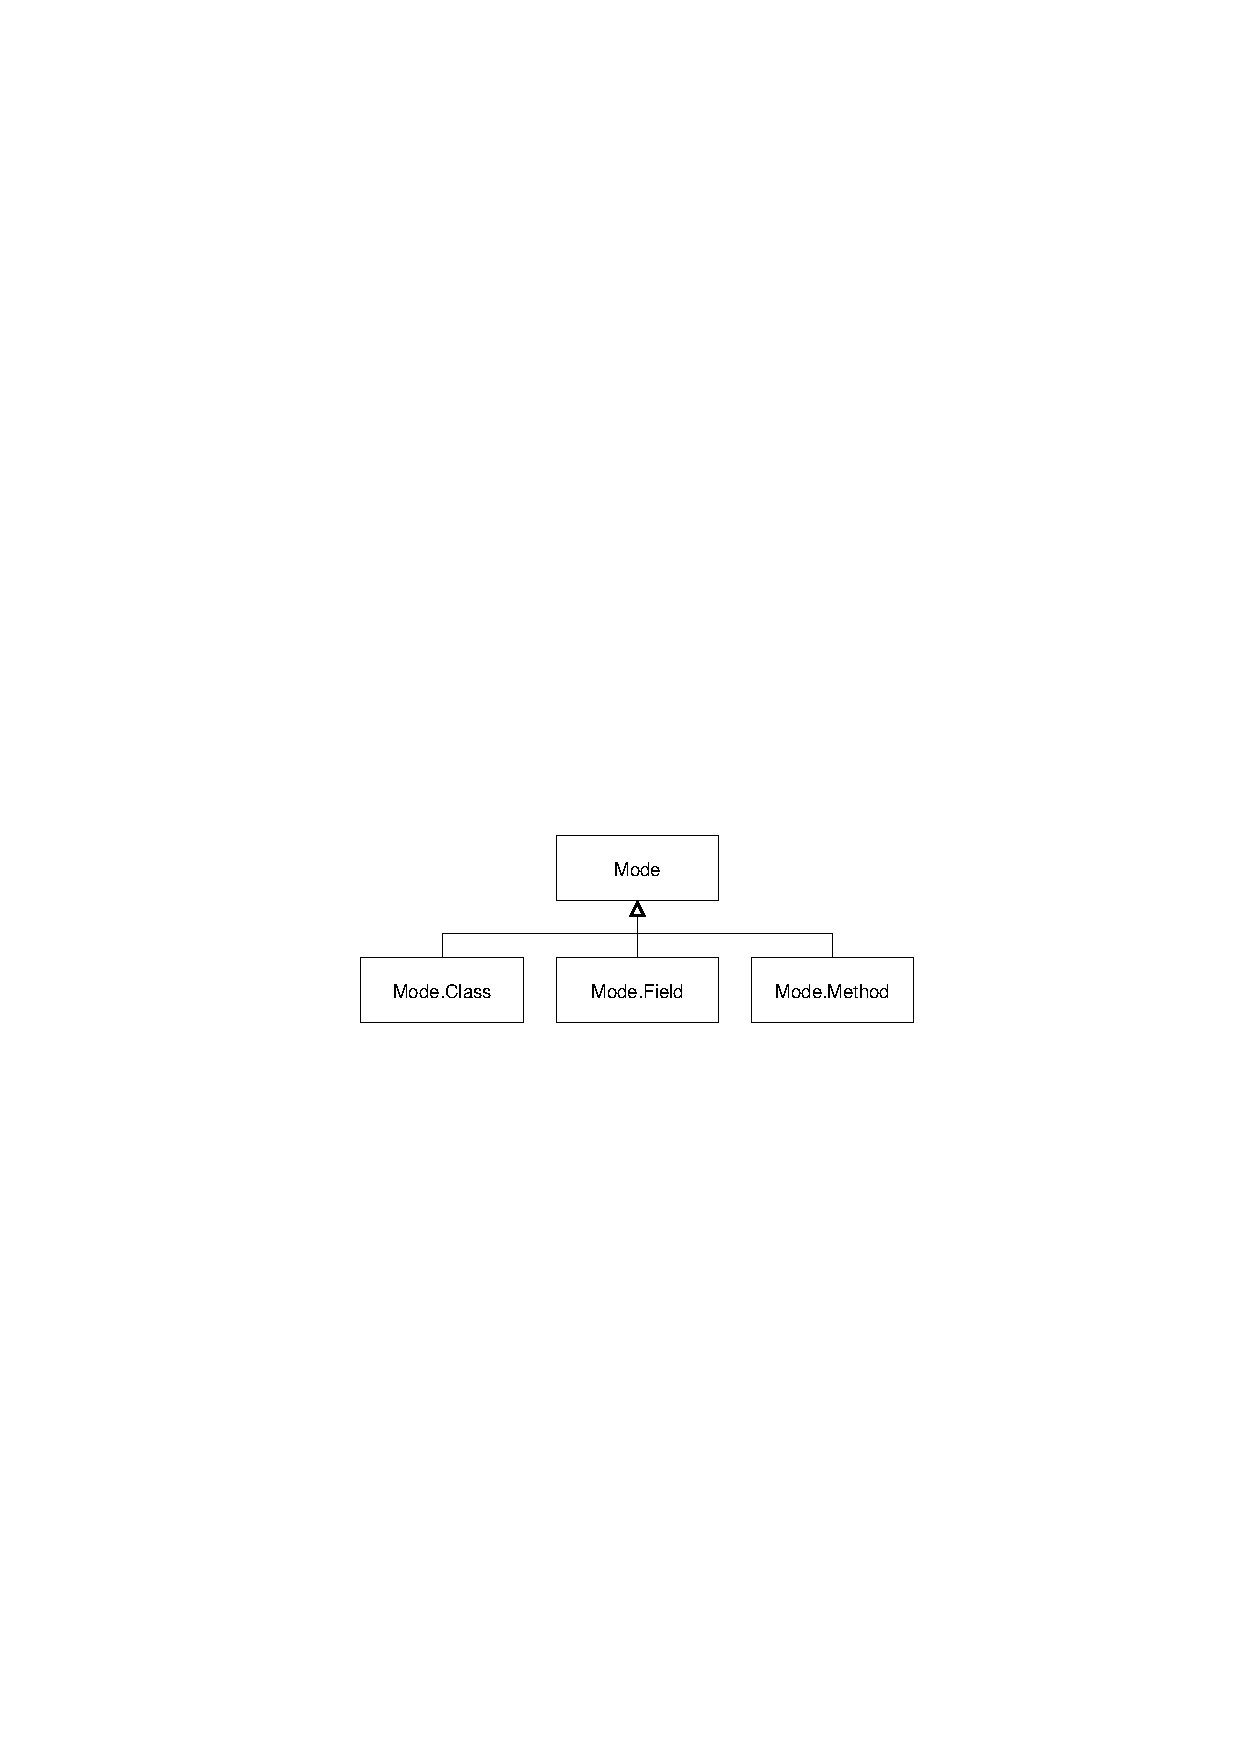
\includegraphics{modehierarchy.epsi}
\caption{The hierarchy of \texttt{Mode} classes}
\label{mode_graphic}
\end{center}
\end{figure}

\section{Repository members and their components}\label{member}

\begin{figure}[htb]
\begin{center}
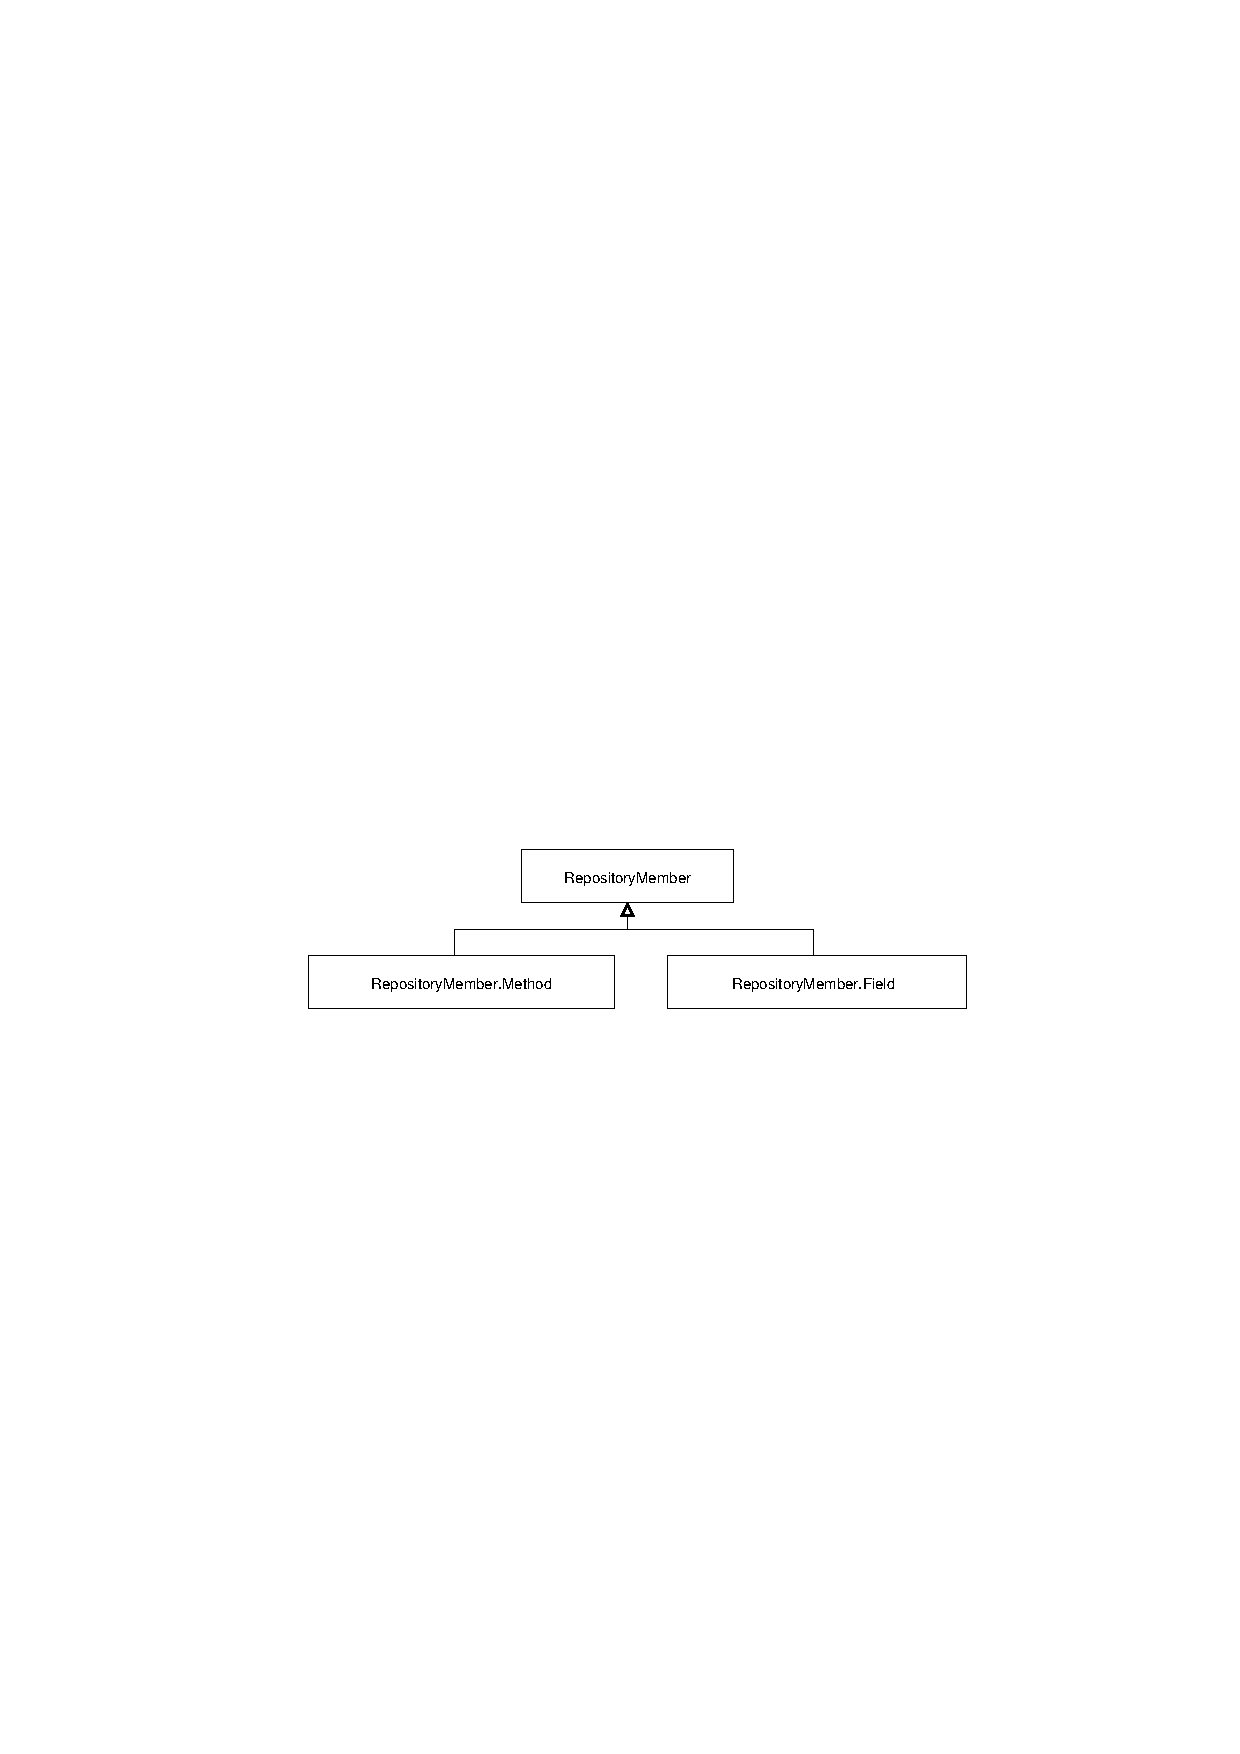
\includegraphics{member_hierarchy.epsi}
\caption{The hierarchy of \texttt{RepositoryMember} classes}
\label{member_graphic}
\end{center}
\end{figure}

The \texttt{RepositoryMember} objects 
(\texttt{Re\-pos\-i\-tory\-Mem\-ber.Field} and 
\texttt{Repository\-Member.Meth\-od}) represent information about 
fields and methods. Each \texttt{Re\-pos\-i\-tor\-y\-Mem\-ber}
object contains at least the following information: the
utf8 index of the member's name (see \S \ref{utf8store}), the
attributes of the member(see \S \ref{attrib}), the modifiers for
that member (see \S \ref{mode}), a \texttt{Descriptor} object,
and an \texttt{Un\-bound\-Se\-lec\-tor} object. 
Descriptors and unbound selectors are described below.

\subsection{Descriptors}

A descriptor captures the type of a method or field.
Descriptors do not uniquely identify a method or field, as many
fields or methods within a class may share the same type. To
uniquely identify a member, a descriptor must be bound to an
unbound selector (see \S \ref{selectors}). Descriptors are
implemented by \texttt{Descriptor} class. The
hierarchy of descriptor classes is shown in figure \ref{desc_graphic}.

\begin{figure}[htb]
\begin{center}
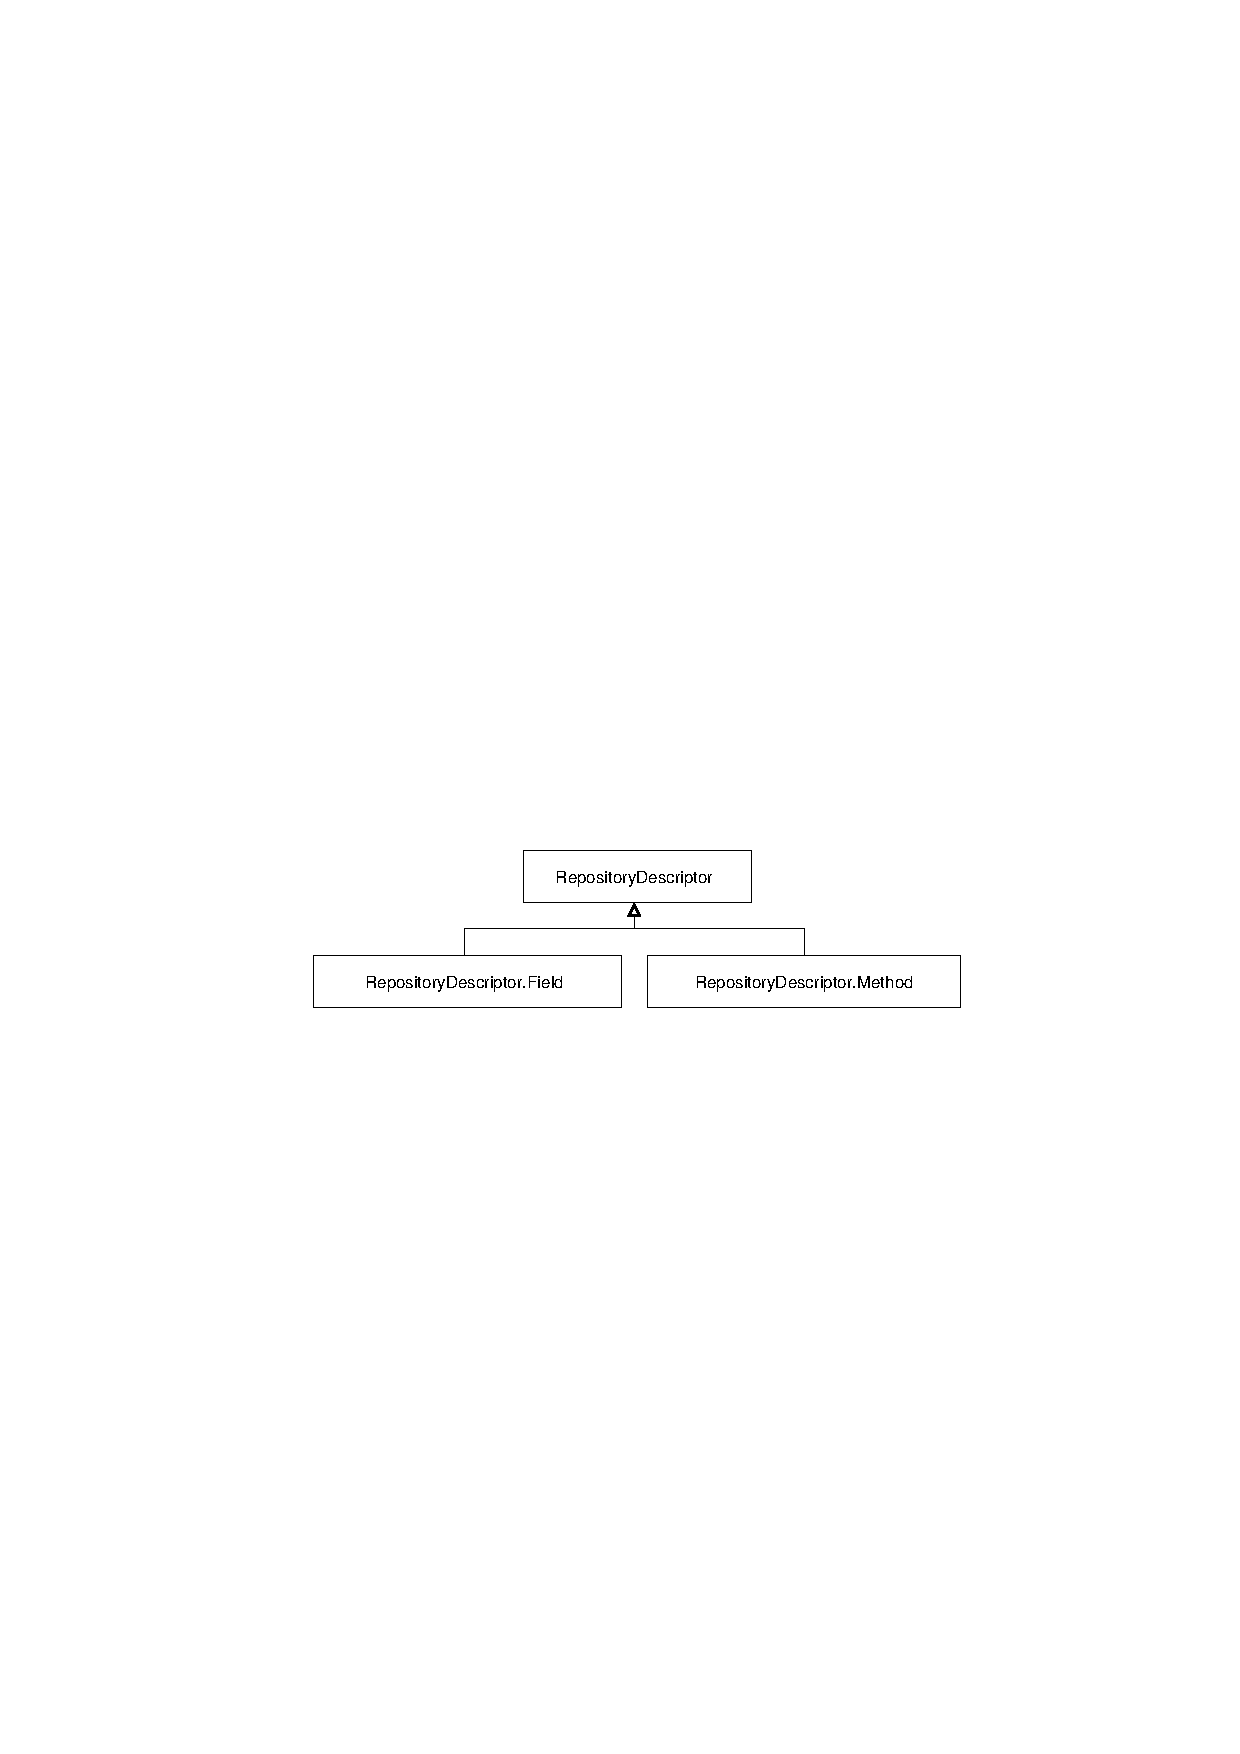
\includegraphics{descriptor_hierarchy.epsi}
\caption{The hierarchy of \texttt{Descriptor} classes}
\label{desc_graphic}
\end{center}
\end{figure}

\subsubsection{Field descriptors}

\texttt{Descriptor.Field} objects
describe field type information. This is merely the
declared type of the field.

\subsubsection{Method descriptors}

\texttt{Descriptor.Meth\-od} objects specify the type of
method objects. A method descriptor contains type 
information about both the method's declared return type and its 
individual declared argument types.

\subsection{Selectors}\label{selectors}

Selectors provide naming information about class members. There are two
types of selectors: bound selectors, and unbound selectors. 
\texttt{Re\-pos\-i\-tory\-Mem\-ber} objects must at least keep a reference to
their unbound selector.

\newpage

\subsubsection{Unbound selectors}\label{unbound}

Unbound selectors denote references to methods and fields consisting of
a pair of a member name and a descriptor. For example the following field 
definition:

\begin{verbatim}

        class Ex {
            int fi;
        }

\end{verbatim}

\noindent is denoted by an unbound selector which indicates that the field's 
name is \texttt{fi} and (through its descriptor) its type is \texttt{I} (for 
\texttt{int}).

\texttt{Un\-bound\-Se\-lec\-tor} objects 
uniquely identify members within a class but do not
necessarily represent all the type information, as they have no reference
to the defining class of the corresponding method or field.

\subsubsection{Bound selectors}

Bound selector objects, or simply \texttt{Se\-lec\-tor}s, represent a binding 
between an unbound selector and a defining class.

Selectors denote references to members consisting of a
defining class \texttt{TypeName} (see \S \ref{typename}) and
an unbound selector. Because this unbound selector, as mentioned in
the previous section, binds a member name to its type information,
a \texttt{Se\-lec\-tor} is effectively a triple consisting of a
member's defining class, name, and descriptor. Thus, if we take
our previous example again:

\begin{verbatim}

        class Ex {
            int fi;
        }

\end{verbatim}

\noindent its bound selector would show that its defining class (through
the defining class \texttt{TypeName}) is \texttt{Ex}, the name of the field
is \texttt{fi} and (through its descriptor) its type is \texttt{I}.

Because of the binding between defining type and member information,
a \texttt{Se\-lec\-tor} uniquely identifies a method or field.

\subsection{RepositoryMember.Field}\label{field}

Each \texttt{RepositoryMember.Field} object represents the information for
one field within a class. In addition to the general requirements for 
\texttt{Re\-pos\-i\-tory\-Mem\-ber} objects, 
\texttt{Re\-pos\-i\-tory\-Mem\-ber.Field} objects also should be able to 
return their constant value bits for non-reference objects. This may mean 
returning the value of a repository utf8 store reference for \texttt{String} 
objects, or the bit sequence defining a primitive type.

%% FIXME: Is what gets returned here implementation dependent?? 

\subsection{RepositoryMember.Me\-thod}\label{method}

\texttt{Re\-pos\-i\-tory\-Mem\-ber.Meth\-od} objects encapsulate the 
information about each member method of a class. 
\texttt{Re\-pos\-i\-tory\-Mem\-ber.Meth\-od} objects must, in addition to the 
general \texttt{Re\-pos\-i\-tory\-Mem\-ber} object functionality, be able to 
return the \texttt{RepositoryCodeFragment} associated with the method. Also, 
they must contain a reference to a list of the \texttt{TypeName} objects for 
declared thrown exceptions of the method.

\subsection{RepositoryCodeFragment}\label{codefrag}

%% FIXME: I'm making this up - still don't understand this really.

FIXME: This is outdated.

A \texttt{RepositoryCodeFragment} contains the code related to a method.
While there are potentially several different kinds of code fragments,
the only one currently supported is the 
\texttt{Re\-pos\-i\-tory\-Byte\-Code\-Frag\-ment} type.

\subsubsection{Code fragments and kinds}

A code fragment is an abstract term for some representation of a set of
instructions. These instructions usually represent the code attached to
a method. Theoretically, there could be several different representations
of the same method's code. Each of these could be of a different
{\em kind}. Currently, the only supported kind is for byte code fragments.

\subsubsection{Byte code fragments}\label{bcf}

Byte code fragments are, as mentioned, specific kinds of code fragments.
\texttt{Re\-pos\-i\-tory\-Byte\-Code\-Frag\-ment} objects contain a byte array 
representing the bytecode, the maximum stack height for the bytecode fragment, 
a local variable table, the number of local variables for the bytecode 
fragment an exception table with entries for each thrown exception, 
and an attribute table for each of the code fragment's attributes. 
Additionally, there is a reference to the associated method's descriptor and 
the constant pool used by the bytecode fragment.

Also potentially associated with a byte code fragment is a line number table,
which is an optional attribute as discussed in \S \ref{attrib}.

\section{Attribute}\label{attrib}

Attributes, as specified in the JVM Specification, \S 4.7, 
must extend the abstract \texttt{Attribute} class. 
There are several different kinds of attributes, each of which will be 
explained in this section.

Attributes are used to provide additional information for various structures
within the class file. Objects that make up the 
\texttt{Re\-pos\-i\-tory\-Class} structure, such as 
\texttt{Re\-pos\-i\-tory\-Mem\-ber} (see \S \ref{member})
and \texttt{RepositoryCodeFragment} (\S \ref{codefrag}) objects, 
mirror this and contain representations of these attributes.

All \texttt{Attribute} objects contain a reference to the
repository utf8 string index for the name of the attribute (see \S
\ref{utf8store} for information about utf8 strings in the repository). 
This name will generally represent the attribute object's type. Additionally,
these objects require a method to convert this name information to a
\texttt{String} object. 

% They should all also contain an \texttt{accept()} method
% for the visitor pattern (see \S \ref{visitor}).
% Cut out for now... since I think this applies to almost everything.

Much of the other information contained within an attribute is specific
to the attribute type, as described in the next section.

\subsection{Attribute Types}\label{atttypes}

There are several different kinds of attributes described in the JVM
Specification. Additionally, there can also be attributes imported from a
third-party. Attribute types and their structure within OVM are described
below.

\subsubsection{Deprecated}

This attribute object requires no specific data structures outside of those
demanded by \texttt{Attribute}. Deprecated attributes are to be 
associated with \texttt{Re\-pos\-i\-tory\-Class}, 
\texttt{Re\-pos\-i\-tory\-Mem\-ber.Field}, and
\texttt{Re\-pos\-i\-tory\-Mem\-ber.Meth\-od} data structures whose use is to 
be discouraged in favor of more recent functionality.

\subsubsection{InnerClasses}

The \texttt{InnerClasses} attribute is present in any 
\texttt{Re\-pos\-i\-tory\-Class} object whose represented class file contains 
constant pool references to classes or interfaces which are 
``not a member of a package'' (JVM Specification, \S 4.7.5). 
In other words, all classes (or interfaces) which contain inner classes 
or interfaces must have this attribute present in their
\texttt{Re\-pos\-i\-tory\-Class} objects.

Contained within this attribute object is a table of inner classes/interfaces
which are members of outer class. Each entry in the table refers to one
inner class. Each inner class entry contains the following information:

\begin{itemize}
	\item the \texttt{TypeName} of this inner class - this represents the
	      simple name of the inner class as it appears within the
	      source file. See \S \ref{typename} for details on
	      \texttt{TypeName} objects.
	\item the outer class \texttt{TypeName} - this is the 
	      \texttt{TypeName} object for the enclosing class of the inner 
	      class specified by this entry. Note that there is no guarantee 
	      that this will be the current repository class; in the case of
	      multiple nested inner classes, the outer class of this
              entry might be another inner class in this attribute's class 
	      file.
%FIXME: Is this true???
	\item the repository utf8 string index of the simple name of this inner
	      class (see \S \ref{utf8store} for utf8 string information)
	\item the \texttt{Mode} object representing the modifiers of this
	      inner class (see \S \ref{mode} for \texttt{Mode} details)
\end{itemize}

The attribute also contains a variable which counts the number of entries in
the table.

\subsubsection{LineNumberTable}

The optional \texttt{LineNumberTable} attribute is associated with a
\texttt{Re\-pos\-i\-tory\-Byte\-Code\-Frag\-ment} object (\S \ref{bcf}) and
maps source file line numbers to the virtual machine's code array.

Each entry within this table corresponds to a new line of code within the 
source file. Entries contain the following information:

\begin{itemize}
	\item the line number at which a new line of source code begins
	\item the \texttt{start\_pc} index for the corresponding line number, 
	      which is an index into the byte code array which indicates where
	      the code for this line of source code begins.
\end{itemize}

The attribute object also implements the functionality necessary to
obtain the line number corresponding to a given offset within the 
byte code. Note that this offset will not necessarily be equal to
any of the \texttt{start\_pc} indices in this attribute's table, but should
fall within the interval covered by one of the line number entries.

\subsubsection{LocalVariableTable}

The \texttt{LocalVariableTable} attribute is an optional attribute associated
with a \texttt{Re\-pos\-i\-tory\-Byte\-Code\-Frag\-ment} object (\S \ref{bcf}).
This attribute maps a method's local variables to current information about 
the variable.

Each entry in the table corresponds to one of the local variables in the
code fragment which owns this attribute. These entries contain the
following information:

\begin{itemize}
	\item the repository utf8 string index for the name of this
	      variable (see \S \ref{utf8store})
	\item a descriptor (see \texttt{Descriptor.Field} in
              \S \ref{field}) for this variable
	\item this entry's index in the local variable table of the current
              frame
	\item the \texttt{start\_pc} index for this variable; this is
              the minimum byte code index at which this variable {\em must}
              have a value
	\item the offset from this entry's \texttt{start\_pc} index which
	      is used to calculate the interval over which this variable
              must have a value
\end{itemize}

The JVM Specification (\S 4.7.9) suggests that this attribute is 
particularly useful for debuggers, which may need to display
a particular variable's value during runtime.

\subsubsection{SourceFile}

This attribute object contains information about the source file from which a 
particular \texttt{Re\-pos\-i\-tory\-Class} object is derived. Only one source
file attribute can be associated with any class representation object, as 
implied by the JVM Specification. \texttt{SourceFile} attribute objects must 
at least have an index to the repository utf8 string representation of the
source file's name, as well as a method to convert this name to a 
\texttt{String}.

\subsubsection{Synthetic}

This attribute, like the \texttt{Deprecated} attribute, requires
no specific additional data structures other than those required through
inheritance from the superinterface. This attribute is used in 
\texttt{Re\-pos\-i\-tory\-Class}, \texttt{Re\-pos\-i\-tory\-Mem\-ber.Field}, 
and \texttt{Re\-pos\-i\-tory\-Mem\-ber.Meth\-od} data structures which that 
are associated with a class representation but do not exist in the original 
source code.

\subsubsection{Third party attributes}

Third party attributes may have many different representations, depending
upon the specific attribute. These attributes are all specified by 
third-parties, not the JVM Specification. Their specification and specific 
structure, then, is completely dependent upon the decisions of the third party.
They must, of course, at least contain the functionality required of all
\texttt{Attribute} objects; all of the attribute's information
(except for name and length) will be contained in a \texttt{byte} array
within the attribute structure.

\section{Arrays}\label{arrays}

There are three important concepts related to arrays which are
used throughout the code: element types, component types, and
depth. To explain these, we use the following Java statement as an example:

\begin{verbatim}

        String[][][] 3D_array = new String[10][12][3];

\end{verbatim}

\begin{description}

	\item[Element Types]
	The {\em element} type is also referred to as the 
	{\em innermost component} type and refers to the type at the
	0th dimension of the array. For the statement above, then, the 
	{\em element} type is \texttt{String}. Most methods in OVM dealing
	with arrays use the name {\em innermost component} to avoid 
	confusion.

	\item[Component Types]
	The {\em component} type refers to the 
	types of what are generally (outside of this context) referred to as 
	array elements; that is, for an $n$-dimensional array, the 
	{\em component} type is the type of the objects at dimension 
	$n-1$. So in our example, the {\em component} type of the array is
	\texttt{String[][]}, or a $2$-dimensional \texttt{String} array.

	\item[Depth] The {\em depth} of an array refers to its 
	number of dimensions.In our example array, this value is $3$. The 
	{\em depth} of an array type is demonstrated by the number of left 
	brackets in its fully-qualified name.

\end{description}

\chapter{Care and Usage of Your New Repository Pet}\label{usage}

%% ok, now that you're done laughing, comment that out and put this in:
%% \chapter{Usage of the Repository}\label{usage}

With an understanding of the composition of the repository, it is now possible
to discuss how the repository is used. This chapter aims to discuss both
general repository usage concepts as well as the access, creation, and usage 
of particular repository components.

\section{General concepts}

Many components of the repository have characteristics which are best
addressed individually. Before this is approached, however, there are
a few mechanisms which are used frequently throughout OVM which should be
explained. Some, such as {\em builders} and {\em factories}, deal
mostly with object creation. Others, like {\em singletons}, regulate
how many objects are maintained in the repository. {\em Visitors} are
used frequently to perform actions upon objects which depend upon object
structure and composition. Finally, we discuss the 
\texttt{Re\-pos\-i\-tory\-Utils} class, which provides static methods for 
manipulating repository objects.

Additionally, we discuss particular issues with comparisons and equality
in OVM and how these affect object usage.

\subsection{Builders and Factories}

{\em Builders} and {\em Factories} are both used throughout OVM as
an interface for object creation. Builders are stateful objects which use
their accumulated state in order to create objects with particular 
characteristics. Factories, on the other hand, are stateless and may rely
on input parameters for customizing object creation. 

The practical result of this is that factory methods do not generally have
to worry about interactions resulting from previous manipulation of the factory
object. The factory may be asked to create objects several different times
with different parameters from different threads and the creation of one
object will not affect the outcome of the creation of other objects. This is
not necessarily true of builders because of their statefulness and should be
considered when using builders.

For example, the builder used to create repository classes has a series of 
{\em get} and {\em set} methods to set class name, members, version numbers,
modifiers, and other class-specific attributes. Once set in the builder,
whenever \texttt{build()} is called via this builder object, a class
with the set attributes is built. These attributes will remain set in
any class built with this builder until the state is reset through the
\texttt{reset()} method.

On the other hand, repository descriptors are created via a factory. The
same factory can be used repeatedly without any need to ``reset'' the
factory object. Instead of setting states within the factory, the necessary
information for object creation is passed to the factory through the
parameters of the \texttt{makeDescriptor()} method. For example, the
field descriptor version of this creation method takes a \texttt{TypeName}, 
and the method descriptor version takes a list of method arguments and the 
\texttt{TypeName} of the return value. No information about these descriptors
is retained within the factory object after creation.

\subsection{Visitors}\label{visitor}

%% FIXME: More of this is kind of made up...

The term {\em visitor} refers to an object that implements the 
\texttt{Visitor} pattern \cite{Gamma1995}. This pattern provides a method of 
traversing an object graph while performing type-specific actions on each 
object via double-dispatch. Practically speaking, this means that nearly every
repository object class contains an \texttt{accept()} method, and several
classes contain methods to visit their components, attributes, etc.
Appropriate visitor classes can then be written to perform actions upon these
object graphs.

There are several visitor interfaces specified within the repository.
\texttt{Re\-pos\-i\-tory\-Vis\-i\-tor} is the general interface for a visitor 
pattern 
defined over repository data structures. \texttt{RepositoryEmptyVisitor}
is an implementation of this interface; as the name suggests, the methods are
empty. This class is useful in that extensions can implement visitor
functionality for only the data structures they want to visit; all other
data structure visits will simply return without further graph traversal.
Thus, only overridden methods have any functionality in extensions to this 
class. \texttt{CloneClassVisitor} is also an implementation of the
\texttt{Re\-pos\-i\-tory\-Vis\-i\-tor} interface and can be used to create a
\texttt{ClassBuilder} which produces \texttt{Re\-pos\-i\-tory\-Class} objects 
which are deep copies of the class object that \texttt{CloneClassVisitor} 
visits. As most repository objects are read-only once created, this form of a 
deep copy can be very useful.

\subsection{Singletons}

Many repository objects are kept as {\em singletons} within the 
repository. When used properly, this guarantees that a particular object 
will not be duplicated in multiple places. For example, it is possible that a
user or application will attempt to create the same \texttt{TypeName}
object in several places; if a \texttt{TypeName} object already exists
for that particular type name, and \texttt{TypeName} objects are
kept as singletons, the object will not be created again.
Instead, the existing object will be returned and used. This is often
implemented using hash tables to store the singleton instance.

Singleton objects are useful for a few reasons. First of all, the overhead
of object creation only needs to be expended once instead of several times.
Secondly, space is often saved by keeping only one copy of the object in
the system instead of several. Finally, the system is made more efficient by
allowing comparisons to take place based upon references instead of upon
deeper equality checks (see \S \ref{equals}).

\subsection{Equality}\label{equals}

Equality checks should be performed with some degree of
caution. Some objects are interned and guaranteed to be singletons; for these
objects, reference equality (i.e. \texttt{a == b}) should be used
in place of \texttt{equals()} methods whenever possible for 
efficiency. However, one must be careful about using reference
equality; some objects, such as \texttt{Mode} objects, are singleton
objects in the reference implementation of OVM, but will not necessarily
be so in all implementations. This emphasizes the importance of
understanding what characteristics are imposed on all implementations,
and which are implementation-specific details.

\subsection{RepositoryUtils}\label{reputils}

The \texttt{RepositoryUtils} class provides static utility methods for 
repository manipulation. This allows applications using a repository to 
manipulate it without knowing repository-specific or implementation-specific 
details. Many of the methods have two variants; one which requires the 
\texttt{Repository} object to be passed in as an argument, and the other
which obtains a repository on its own.

There are a variety of access, creation, and manipulation methods in this 
class. The following is a brief description of each method, and how it is
used:

\begin{description}

	\item[getSystemClass] This method is used to retrieve the 
	\texttt{Re\-pos\-i\-tory\-Class} representation of a system class or 
	interface. There are two variants of this method: one
	requires a \texttt{String} describing the package of a system class
	(e.g. \texttt{java.util}) and another \texttt{String} describing the 
	simple name of the class (e.g. \texttt{Hashtable}), and the other is
	used specifically for classes within the \texttt{java.lang} package and
	requires only the simple name of the class (e.g. \texttt{Object})
	as a \texttt{String}.

	\item[makeTypeName] Given a \texttt{String} object containing
	the fully-qualified name (e.g. \texttt{Ljava/lang/Object;}) for
	a type, this method returns a corresponding \texttt{TypeName} object.
	See the JVM Specification, \S 2.7.5, for more information
	on fully-qualified names.

	\item[makeUnboundSelector] This method requires a \texttt{String}
	object which describes the name and descriptor information for a
	selector and returns a 
	\texttt{Re\-pos\-i\-tory\-Un\-bound\-Se\-lec\-tor} object. See \S 
	\ref{compunbound} for information about the format of this string.

	\item[methodSelectorFor] This method will, given both a \texttt{String}
	object containing the fully-qualified name of a defining class
	and a second \texttt{String} object containing unbound method selector
	information, return a bound selector object 
	(\texttt{Se\-lec\-tor.Meth\-od}) representing the binding between a 
	defining class, and a method's name and type information. See \S 
	\ref{compunbound} for information on unbound selector string format.

	\item[fieldSelectorFor] This method has the same functionality and
	usage as \texttt{meth\-od\-Se\-lec\-tor\-For} does, except for the 
	usage of a \texttt{String} containing unbound {\em field} selector 
	information and the return of a bound field selector 
	(\texttt{Se\-lec\-tor.Field}) object. Please see \S 
	\ref{compunbound} and \S \ref{compdesc} for an understanding of 
	how method and field unbound selector input strings will differ.

	\item[selectorFor] This method performs the same tasks as
	\texttt{field\-Se\-lec\-tor\-For} and 
	\texttt{meth\-od\-Se\-lec\-tor\-For}, but for generic unbound selector 
	input strings. Practically, this simply means that the user doesn't 
	necessarily have to differentiate between bound method and field 
	selectors when creating them via \texttt{Re\-pos\-i\-tory\-Utils} 
	methods; rather the code can distinguish between the two and 
	automatically produce the correct \texttt{Se\-lec\-tor} type. 
	Formats correspond to those used for \texttt{field\-Se\-lec\-tor\-For} 
	and \texttt{meth\-od\-Se\-lec\-tor\-For}.

\end{description}

\section{Component Usage}

This section contains information which deals with component-specific
usage details. Many components have characteristics within the repository,
such as being maintained as singletons or being referenced by index, which
are important to take notice of and which can often be used advantageously.

\subsection{utf8 Strings}

Utf8 strings, as mentioned in \S \ref{utf8store}, are kept in the
repository and referenced via an \texttt{int} index into the utf8
store. Repeated occurances of a given string within the repository
will map to the same utf8 store index. Strings that exist within the
utf8 store are said to be {\em installed} there; thus, the
utf8 store contains methods which allow both string installation and 
retrieval of strings within the repository. Utf8 strings can be stored
from \texttt{ByteArray} objects or primitive byte arrays via the
\texttt{installUtf8()} methods. Utf8 strings can be retrieved in
primitive byte array format, given a string's index in the utf8 
store, via the \texttt{getUtf8()} method, or as a \texttt{String} object
via the \texttt{getUtf8AsString()} method. 

Utf8 strings can be written to output streams and \texttt{Byte\-Buff\-ers} as
well. The \texttt{writeUtf8()} method will write the stream to either the
specified \texttt{Out\-put\-Stream} object or \texttt{Byte\-Buff\-er} object 
when given the utf8 string index.

Given a primitive byte array, it is also possible search the repository for 
the index of a utf8 sequence which matches a given portion of the input byte 
array.

Finally, the length of a utf8 string can be found via its index and the
\texttt{getUtf8Length()} method.

\subsection{TypeName}

\texttt{TypeName} objects can be created through the
\texttt{Re\-pos\-i\-tory\-Utils.make\-Type\-Name()} method (see \ref{reputils})
and through \texttt{TypeName.Fac\-tory} implementations.

\texttt{TypeName.Fac\-tory} implementations contain functionality
to make \texttt{TypeName} objects of various types in various ways.
As with \texttt{Re\-pos\-i\-tory\-Utils.make\-Type\-Name()}, there are factory 
methods to create typenames given a representation of the type's 
fully-qualified name (in this case, within a \texttt{Byte\-Buff\-er} - see JVM 
Specification \S 2.7.5 for information on fully qualified names). Additionally,
\texttt{TypeName} objects can be created given either \texttt{String}
representations of package names and class simple names, or the
repository utf8 string indexes to representations of these names.
Finally, \texttt{TypeName.Array} objects for array typenames can be
created via three different versions of \texttt{make\-Type\-Name()}.
Two of these are straightforward and only require either a primitive or scalar
\texttt{TypeName} object representing the {\em element} type of the array
(see \S \ref{arrays}) and the number of dimensions of the desired
array. The third variation differs in that the \texttt{TypeName} object
passed in is only guaranteed to be a compound (i.e. non-primitive)
typename. The consequence of this is that the \texttt{TypeName} object
passed in could already be an array; if this is the case, the number
of dimensions in the input argument is {\em added} to the number
of dimensions in the \texttt{TypeName.Compound} parameter in creating
the new \texttt{TypeName}. The returned array typename will contain the
same element type as the original typename, as would be expected.

Typenames are interned within the repository; as such, repeated calls
to \texttt{make\-Type\-Name()} methods for the same typename should return a
single, unified reference. This means, practically, that for comparisons,
equality by reference should be computed instead of using \texttt{equals()}
methods or other measures of deeper equality. Once a typename has been created,
\texttt{make\-Type\-Name()} effectively functions as a retrieval method.

Note that the typename for the root of the object hierarchy (e.g.
the typename for \texttt{java.lang.Object}), as well as the typename objects
for primitive types, are created and interned at repository creation time.
Practically speaking, this means that the user should not need to explicitly
create these types. Thus, only accessor methods (\texttt{getRoot()},
\texttt{getPrimitiveTypeName()}) are provided. The primitive typename accessor
method takes as its argument a tag which is the corresponding
\texttt{TypeCodes} constant for that primitive type (see \S
\ref{typecodes}).

\subsection{Descriptor}\label{compdesc}

\texttt{Descriptor} objects are, like many repository objects, 
interned in the repository, allowing for reference equality checks. It is
possible to create or retrieve a descriptor via a number of kinds of input.
These will all be described in this section; however, because there are a 
number of places in the repository where a character-based representation of a 
descriptor may be used as input or output, the way in which these
\texttt{Strings}, \texttt{Byte\-Buff\-ers}, byte arrays, etc.) are formatted is
described first. These representations are described by a grammar, which is
explained below.

\subsubsection{Grammar}

The following grammar is taken from \S 4.3 of the JVM Specification;
it describes the format of descriptors when input via \texttt{Byte\-Buff\-ers},
\texttt{Strings}, and byte arrays. This is also the format of descriptors
when returned in similar character representations or written to streams.

For fields:
\begin{verbatim}

     FieldDescriptor: FieldType
     ComponentType: FieldType
     FieldType: BaseType | ObjectType | ArrayType
     BaseType: B | C | D | F | I | J | S | Z
     ObjectType: L<classname>;
     ArrayType: [ComponentType
     <classname>: (fully qualified class or interface name)

\end{verbatim}
For methods:
\begin{verbatim}

     MethodDescriptor: (ParameterDescriptor*)ReturnDescriptor
     ParameterDescriptor: FieldType
     ReturnDescriptor: FieldType | V
                       (where V is for void return types)
\end{verbatim}

So, for example, the descriptor for a field of type \texttt{boolean} would have
a descriptor string format of \texttt{Z}, whereas a field of type
\texttt{java.util.HashMap} would have a descriptor string format of
\texttt{Ljava.util.HashMap;}.

Similarly, a method declared as follows:
\begin{verbatim}

public void foo(int a, String[] b) {}

\end{verbatim}
\noindent
would have a descriptor that looks like this: \texttt{(I[Ljava.lang.String;)V}

\subsubsection{Creation and Retrieval}
Because descriptors are interned, multiple references to identical
descriptors are guaranteed to lead to one single descriptor. As such,
the \texttt{makeDescriptor()} methods of implementations of
\texttt{Descriptor.Fac\-tory} can either create new descriptors
or retrieve existing ones. 

The version of \texttt{Descriptor.makeDescriptor()} that takes
a \texttt{Byte\-Buff\-er} description of a descriptor as input conforms
to the grammar described above.

The other versions of the method correspond to the specific type information
for methods and fields; the method flavor takes the \texttt{TypeName} of
the return value's type along with a \texttt{List} of the \texttt{TypeName}
objects of the arguments. The field version takes only the declared field
type's \texttt{TypeName} object.

\subsection{Unbound selector}\label{compunbound}

\subsubsection{Creation and retrieval}

Unbound selectors can also be created and retrieved from either the 
\texttt{Re\-pos\-i\-tory\-Utils} creation method 
(\texttt{Re\-pos\-i\-tory\-Utils.make\-Un\-bound\-De\-scrip\-tor}), or from the
\texttt{make\-Un\-bound\-De\-scrip\-tor()} method in 
\texttt{Un\-bound\-Se\-lec\-tor.Fac\-tory}. Both methods take
arguments in the format described for strings below; the 
\texttt{Re\-pos\-i\-tory\-Utils} version takes a \texttt{String}, whereas the 
factory method takes a \texttt{Byte\-Buff\-er}.

\subsubsection{String format}

Unbound selectors can be represented (in input or output) using a string 
in the following format:
\begin{verbatim}
      <name> ':' <descriptor string>
\end{verbatim}
\noindent The descriptor string format is described in \S \ref{compdesc}.

\subsection{Bound selector}

Bound selectors (i.e. \texttt{Se\-lec\-tor} objects) can be created through
either the \texttt{Re\-pos\-i\-tory\-Utils} methods 
(\texttt{meth\-od\-Se\-lec\-tor\-For()}, \texttt{field\-Se\-lec\-tor\-For()}, 
or \texttt{selectorFor()}), or through the \texttt{makeSelector()} methods 
in \texttt{Se\-lec\-tor.Fac\-tory}. The \texttt{makeSelector()} methods take 
the unbound selector of the field or method along with the type name object of
its defining class. The \texttt{Re\-pos\-i\-tory\-Utils} methods function as 
defined in \S \ref{reputils}.

\subsection{Attributes}

Attributes can be declared in the \texttt{RepositoryBuilder} object which
creates the associated class, method, field, or code object. There are
several methods for declaring these attributes in builders. There are
two versions of the \texttt{declareAttribute()} method: the first is a
generic attribute declaration method and takes a \texttt{Attribute}
object as an argument. The second is for third-party attributes and takes
the repository utf8 string index of the attribute name as well as a byte
array containing the attribute's content. There are three more specific
attribute declaration methods (\texttt{declareDeprecated()}, 
\texttt{de\-clare\-Syn\-thet\-ic()}, and \texttt{declareSourceFile()}) which
add \texttt{Deprecated}, \texttt{Syn\-thet\-ic}, and \texttt{SourceFile}
attributes respectively. Attributes can be retrieved from a method, field,
class, or code object through that object's \texttt{getAttributes()} method.
This method will return an array containing the object's attributes.

\subsection{Mode objects}

Mode objects, in the default implementation, are singletons. This is not 
enforced for all implementations, however, and care should be taken not
to make this assumption without knowing the underlying details.

\subsubsection{Creation and Retrieval}
\texttt{Mode} objects are created and retrieved in two ways: through 
\texttt{Mode.Fac\-tory} methods, and through builders created by
\texttt{make\-Meth\-od\-Build\-er()}, \texttt{make\-Field\-Build\-er()}, and
\texttt{make\-Class\-Build\-er()}. These builder creation methods return
builders whose modifier bits can be set such that they can build
specific \texttt{Mode} objects with those modifiers.

\subsubsection{Usage}

Once created, \texttt{Mode} objects can then be tested for individual
modifiers by querying the individual object. \texttt{Mode} objects should
be able to answer queries for modifiers which are valid for the type
of object being modified. Thus, given a \texttt{Mode.Field} object 
\texttt{foo}, to find out if \texttt{foo} contains the modifier for a
static field, we can call \texttt{foo.isStatic()} and find out if
the modifier set contained in the object includes the \texttt{static}
modifier. 

\subsection{RepositoryMember usage details}

\texttt{Re\-pos\-i\-tory\-Mem\-ber} objects (\texttt{Field} and 
\texttt{Method}) can be retrieved through the \texttt{Re\-pos\-i\-tory\-Class}
objects they belong to. (See \S \ref{repclass_usage} for more information
on how to retrieve \texttt{Re\-pos\-i\-tory\-Mem\-ber} objects) They are 
created through builders specific to \texttt{Re\-pos\-i\-tory\-Mem\-ber.Field} 
and \texttt{Re\-pos\-i\-tory\-Mem\-ber.Meth\-od}. All 
\texttt{Re\-pos\-i\-tory\-Mem\-ber} objects have certain functionality in 
common. Member names (as \texttt{String} objects) can be retrieved through the 
\texttt{getName} method, and the repository utf8 indices of names is returned 
by the \texttt{getNameIndex} method. The array of associated attributes can be 
retrieved through the \texttt{getAttributes} method, and the generic descriptor
object for a member can be obtained through the \texttt{getUnrefinedDescriptor}
method. Similarly, the generic member mode object can be obtained through 
\texttt{getUnrefinedMode}.

Specific details of member types are discussed below.

\subsubsection{Field-specific usage details}

Field-specific components can be retrieved through methods in 
\texttt{Re\-pos\-i\-tory\-Mem\-ber.Field}. Field mode objects are obtained 
through \texttt{getMode}, field descriptor objects are obtained through
\texttt{getDescriptor}, and field unbound selector objects are obtained
through \texttt{getUnboundSelector}. A field's constant value can be
retrieved as an object through the \texttt{getConstantValue} method,
and as a set of bits stored in a \texttt{long} value from the
\texttt{getConstantValueBits} method.

For field builders, all of these values can be set through corresponding
set methods before creating a field object.

\subsubsection{Method-specific usage details}

Method-specific components can be obtained from methods similar to
those in \texttt{Re\-pos\-i\-tory\-Mem\-ber.Field}. 
\texttt{Re\-pos\-i\-tory\-Mem\-ber.Meth\-od} contains \texttt{getMode}, 
\texttt{getDescriptor}, and \texttt{getDescriptor} methods. Additionally, 
there is method-specific functionality. Code fragments can be obtained through 
the \texttt{get\-Code\-Fragment} method, which can either be argumentless, or 
they can take a \texttt{Re\-pos\-i\-tory\-Code\-Frag\-ment\-Kind} object to 
retrieve a particular type of code fragment if there is more than one 
representation of the method's code. The \texttt{TypeName} objects for all 
declared thrown exceptions for the method can be returned as an array by 
\texttt{getThrownExceptions}, and a boolean value displaying whether or not 
the method is a constructor will be returned by \texttt{isConstructor}.

As with fields, most of the get methods above are replaced by corresponding
set methods in the builder. Names can be set via \texttt{setName} with
the appropriate utf8 index (note that the builder also contains a
\texttt{getName} method in order to see which method is being built
with the builder). There is a similar get/set pair in the builder for
descriptors (\texttt{getDescriptor} and \texttt{setDescriptor}) and
for modes (\texttt{getMode} and \texttt{setMode}). Thrown exceptions
can be declared in the builder by submitting the \texttt{TypeName} of the 
exception to \texttt{declareThrownException}.

\subsection{RepositoryClass objects}\label{repclass_usage}

%FIXME: Retrieval??

\subsubsection{Usage}

\texttt{RepositoryClass} objects contain several methods to retrieve
class components. The \texttt{TypeName} object for the class's name can
be retrieved through {getName}. For array classes (if \
texttt{Re\-pos\-i\-tory\-Class} objects are supported for array classes in 
the implementation), the \texttt{TypeName} of the component type can be 
retrieved through \texttt{getComponentType}. Modifiers ({\em not} only access
modifiers) can be retrieved from \texttt{getAccessMode}, and an array of 
associated attributes can be obtained through \texttt{getAttributes}. The 
\texttt{TypeName} objects for directly implemented interfaces is returned as 
an array by \texttt{getInterfaces}; note that this does not include interfaces
implemented through inheritance! Also, the super class's \texttt{TypeName}
is retrieved through \texttt{getSuper} (this is self-referential for the
root of the class hierarchy), and the \texttt{TypeName} objects for each
member of the linkset are available through \texttt{getLinkSet}.

There are several methods to access member objects (in this case, methods, 
fields, and inner classes) or various representations thereof. To 
obtain member objects as sets (as opposed to retrieving specific member objects
by selector or name string), the following methods are used:
\begin{description}

	\item[\texttt{getStaticMethods}] returns an array of 
	\texttt{Re\-pos\-i\-tory\-Mem\-ber.Me\-thod} objects representing the 
	class's static methods

	\item[\texttt{getInstanceMethods}] returns an array of 
	\texttt{Re\-pos\-i\-tory\-Mem\-ber.Me\-thod} objects representing the 
	class's instance methods

	\item[\texttt{getStaticFields}] returns an array of 
	\texttt{Re\-pos\-i\-tory\-Mem\-ber.Field} objects representing the 
	class's	static fields

	\item[\texttt{getInstanceFields}] returns an array of 
	\texttt{Re\-pos\-i\-tory\-Mem\-ber.Field} objects representing the 
	class's	instance fields

	\item[\texttt{getStaticInnerClasses}] returns an array of 
	\texttt{TypeName.Scalar} objects corresponding to the
	class's static inner classes

	\item[\texttt{getInstanceInnerClasses}] returns an array of 
	\texttt{TypeName.Scalar} objects corresponding to the
	class's instance inner classes

\end{description}

\noindent Additionally, the \texttt{TypeName.Scalar} object corresponding to 
the class's outer class (if any) is available through the \texttt{getOuter}
method. While this method will return \texttt{null} if there is no
outer class, this can also be determined by calling the \texttt{isInner}
method.

Specific fields and methods can be retrieved through the \texttt{getField}
and \texttt{getMethod} methods. Both have two variants; one takes a
\texttt{String} corresponding to the %FIXME: name? selector?
name of the member, and the other one takes an unbound selector
object for the method or field. Both return the appropriate 
\texttt{Re\-pos\-i\-tory\-Mem\-ber} object.

Finally, the constant pool used by this class can be retrieved via 
\texttt{get\-Con\-stant\-Pool}, and the major and minor versions of the class
file format are available through \texttt{getMajorVersion} and 
\texttt{getMinorVersion}, respectively.

\subsubsection{Creation}

\texttt{RepositoryClass} objects, like most repository objects, are
created through the appropriate builder. It is possible to create a builder 
initialized to the contents of an existing class by calling the 
\texttt{getBuilder} method on the existing class's 
\texttt{Re\-pos\-i\-tory\-Class} object. In the generic case, however, 
components and characteristics must be set individually in the builder.

Class names can be set by the \texttt{setName} method, 
using a \texttt{TypeName.Scalar} as the argument. The 
\texttt{setSuperClassName} and \texttt{setOuterClassName} methods work in
the same manner. Declared implemented interfaces are similarly added
to the builder (one at a time) via \texttt{declareInterface}. Classes
referenced by the bytecode of the class are set in the builder
by sending their \texttt{TypeName.Compound} objects (again, one at a time)
through \texttt{declareReferencedClass}.

Modifiers are set via the \texttt{setAccessMode} method
and take a \texttt{Mode.Class} object, and class file versions are set
either together using the \texttt{setVersions} method, or separately
using the \texttt{setMajorVersion} and \texttt{setMinorVersion} methods.

Class members can be individually declared via \texttt{declareMethod}
and \texttt{de\-clare\-Field}, each of which takes the appropriate
\texttt{Re\-pos\-i\-tory\-Mem\-ber} object. Methods can be additionally
redeclared (replaced with a new method if the old method exists in the
class, or added if it does not) and removed via 
\texttt{re\-de\-clare\-Meth\-od}
and \texttt{removeMethod}. Note that if \texttt{declareMethod} or
\texttt{de\-clare\-Field} is used twice with the same method or field,
a \texttt{RedeclarationError} will be thrown.

Inner classes can be set in two ways. Instance and static inner classes of
this class can be added individually via the \texttt{declareInstanceInnerClass}
and \texttt{declareStaticInnerClass} functions. Both of these take a scalar
typename object as an argument. The other method of setting inner classes
is to declare an inner classes attribute via \texttt{declareInnerClasses}. 
This takes, as arguments, the scalar type name objects for all of the inner 
classes declared or inherited by this class, the scalar type names of their 
corresponding outer classes, and the corresponding \texttt{Mode.Class} 
repository utf8 short name indices for each inner class.
%FIXME: do these get added to the attribute? how do the first variation
%of methods store the typenames? Do they modify the attribute?

Finally, the constant pool used by the class can be declared with 
\texttt{de\-clare\-Con\-stant\-Pool} and takes a 
\texttt{Con\-stant\-Pool} object as its argument.

\chapter{Definitions}\label{defs}

\begin{description}
	\item[access modifiers] Access modifiers determine the access
	rights of objects trying to access the modified class, field, or method
	object. The access modifiers are \texttt{public}, \texttt{default}
	(i.e. package-scoped), \texttt{protected} and \texttt{private}. Not all
	modifiers are access modifiers.

	\item[attribute] Attributes are attached to class, code, field, 
	and method data structures and represent various aspects of these 
	structures. Several types of attributes are defined in the JVM 
	Specification, but there is also the possibility of using user-defined
	or third-party attributes.

	\item[bound selector] A {\em bound selector} encapsulates the
	binding between an {\em unbound selector} and a 
	{\em defining class}. The unbound selector contains information
	about a field or method name and its corresponding type information
	via its {\em descriptor}.

	\item[builder] A stateful object whose purpose is to build objects
	of a particular type. The state determines how objects will
	be built and is maintained by the builder until the state is
	reset.

	\item[bundle] A logical grouping of classes which determine where
	a \texttt{Re\-pos\-i\-tory\-Class} object is to be found at resolution
	time. (see {\em domain}).

	\item[bytecode fragment] A bytecode fragment is a representation
	of the bytecode contained in a method, along with associated
	code attributes, local variable information and tables, stack size,
	and other relevant code-related information.

	\item[code fragment] A representation of the code contained in a
	method. Code fragments can be of various {\em kinds}, which
	specify the type of code fragment used. Currently, the only
	supported kind is that of bytecode fragment. See {\em bytecode
	fragment}, {\em code fragment kind}.

	\item[code fragment kind] The {\em kind} of a code fragment simply
	determines what type of code fragment it is. Currently, only
	bytecode fragments are supported.

	\item[component type] The {\em component type} of an array
	is the type of the object or primitive contained in the array.
	That is, given an $n$-dimensional array, the type of the object
	(or primitive) at dimension $n-1$ is the component type. For
	example, given an array of type \texttt{Object[][]}, its
	component type is of type \texttt{Object[]}.

	\item[compound type names] A compound type name is the type name
	object for any non-primitive type. See {\em TypeName},
	{\em primitive type names}.

	\item[defining class] The class in which a given method or field is 
	declared.

	\item[depth (of an array)] The number of dimensions in an array. For
	example, an array declared as having type \texttt{String[][]} has
	a depth of $2$.

	\item[descriptor] A descriptor encapsulates the type information for
	a field or method. Field descriptors contain the declared field type,
	whereas method descriptors contain the method's declared argument
	and return types. These types are all represented as \texttt{TypeName}
	objects within the descriptor object.

	\item[domain] Domains are application spaces. Objects in different
	domains should have no interaction via shared objects.

	\item[element type] Also known as the {\em innermost component
	type}, the {\em element} type of an array is the type of the
	object (or primitive) at its $0$th dimension. For example, given
	an array of type \texttt{int[][][]}, its element type is \texttt{int}.

	\item[enclosing class] For inner classes, the enclosing class for
	an inner class is the direct outer class. (FIXME: I think! Check this 
	out and explain more)

	\item[factory] A stateless object used for object creation. 
	Characteristics of the created object are obtained via 
	parameter-passing instead of through state maintained by the
	factory. This is in contrast to {\em builders}.

	\item[fully-qualified name] A naming convention for all classes,
	interfaces, and packages as specified in the JVM Specification,
	\S 2.7.5.

	\item[innermost component type] See {\em element type}.

	\item[kind] See {\em code fragment kind}.

	\item[linkset] The set of types required by the implementation
	of a class.

	\item[\texttt{Mode}] {\em Mode} objects represent the modifiers
	of a particular class, interface, field, or method. 
	See {\em modifiers}.

	\item[modifiers] Modifiers are immutable properties associated
	with a class, interface, field, or method. These include
	access modifiers, which describe which other classes can
	access the modified class, interface, field, or method, as well
	as other modifiers which describe properties such as
	\texttt{static}, \texttt{syn\-chron\-ized}, \texttt{final},
	\texttt{transient}, and \texttt{volatile}. 
	See also {\em access modifiers}.

	\item[nested type names] Nested type names are scalar type names
	which represent inner classes and interfaces. See 
	{\em scalar type names}, {\em TypeName}.

	\item[primitive type names] Primitive type names are the type
	name objects associated with primitive types (e.g. \texttt{int},
	\texttt{boolean}, etc.). See {\em TypeName}.

	\item[repository] The repository is a structure contains which an 
	object-oriented representation of the information contained
	in class files and contains the bytecode of all of the classes 
	loaded in a virtual machine.

	\item[\texttt{RepositoryByteCodeFragment}] The repository 
	representation of a method's byte code and its associated information.
	See {\em byte code fragment}.

	\item[\texttt{RepositoryClass}] The repository data structure which 
	represents all of the information obtained by parsing an individual 
	Java class file.

	\item[\texttt{RepositoryCodeFragment}] The repository data structure
	associated with various representations of a method's code.
	See {\em code fragment}.

	\item[\texttt{RepositoryCodeFragmentKind}] The repository interface
	which much be implemented by each unique type of code fragment.
	See {\em code fragment kinds}.

	\item[\texttt{RepositoryMember}] The repository object for class 
	members	such as methods and fields within a 
	\texttt{Re\-pos\-i\-tory\-Class}.

	\item[\texttt{RepositoryMember.Field}] The repository object for fields
	within a \texttt{Re\-pos\-i\-tory\-Class}.

	\item[\texttt{RepositoryMember.Method}] The repository object for 
	methods	within a \texttt{Re\-pos\-i\-tory\-Class}.

	\item[scalar type names] Scalar type names are all type names for
	any non-primitive, non-array type. See {\em TypeName}.

	\item[selector] Selectors are divided into two categories:
	{\em unbound selectors}, which extend the abstract
	\texttt{Un\-bound\-Se\-lec\-tor} class, and 
	{\em bound selectors}, which extend the abstract \texttt{Se\-lec\-tor}
	class. Unbound selectors encapsulate the name and type information 
	of a field or method, whereas bound selectors bind this information to 
	the method or field's {\em defining class}.

	\item[simple name] The name for a class as stated in its class
	file. For instance, the simple name for an object of type
	\texttt{java.lang.Object} is \texttt{Object}.

	\item[singleton] A unique object in a system, of which there are
	no duplicates.

	\item[\texttt{TypeCodes}] The one-character representation
	of an object or primitive's type. For instance, integers are
	represented by \texttt{I}, reference objects by \texttt{L},
	and arrays by \texttt{[}.

	\item[\texttt{TypeName}] \texttt{TypeName} objects are singleton
	objects representing the name associated with a class or
	interface. These objects contain references to both the simple
	name and the fully-qualified name of the class or interface.
	See {\em simple name} and {\em fully-qualified name}.

	\item[\texttt{TypeName.Compound}] The \texttt{TypeName} object for
	non-primitive types. See {\em compound type names}.

	\item[\texttt{TypeName.Nested}] The \texttt{TypeName} object for
	nested types (i.e. inner classes and interfaces). See {\em nested 
	type names}.

	\item[\texttt{TypeName.Primitive}] The \texttt{TypeName} object for
	primitive types. See {\em primitive type names}.

	\item[\texttt{TypeName.Scalar}] The \texttt{TypeName} object for 
	non-primitive, non-array types. See {\em scalar type names}.

	\item[\texttt{TypeName.WidePrimitive}] The \texttt{TypeName} object
	for wide (two-word) primitive types (e.g. \texttt{long}, 
	\texttt{double}). See {\em primitive type names}.

	\item[unbound selector] An unbound selector contains both a 
	representation of a field or method name and the field or method's
	type information via its {\em descriptor}. It is referred to
	as {\em unbound} because it does not contain any reference to
	the field or method's {\em defining class}.

	\item[utf8 store] The utf8 store is an object used for storage and 
	retrieval of utf8 character strings within the repository. See
	{\em utf8 String}.

	\item[utf8 string] Utf8 strings are the storage representation for 
	strings within the repository.

	\item[visitor] An object which traverses an object graph while 
	performing type-specific actions on each object via double-dispatch.

\end{description}

{\small
\bibliographystyle{plain}
\bibliography{rep_refs}
}


\end{document}
